% Lead: Leanne
\section{On-Sky Commissioning Campaign \label{sec:on_sky_campaign}}

The first Rubin on-sky commissioning campaign was conducted using the \gls{LSSTComCam} between \campaignstartdate and \dponeenddate, spanning a total of \nnightscomcam nights.
The primary objective was to optically align the Simonyi Survey Telescope and verify its ability to deliver acceptable image quality using \gls{LSSTComCam}.
In addition, the campaign provided valuable operations experience to facilitate commissioning the full \gls{LSSTCam}, \citep{2024SPIE13096E..1SR,2024SPIE13096E..1OL}.
It is important to note that commissioning \gls{LSSTComCam}  was not an objective of the campaign.
Instead, LSSTComCam was used as a tool to support broader observatory commissioning, including early testing of the \gls{AOS} and the LSST Science Pipelines.
As a result,
% instrument-specific investigations,  such as verifying the pointing model and studying the stray light were deprioritized.
many artifacts present in the data are specific to \gls{LSSTComCam} and will only be addressed if they persist with \gls{LSSTCam}.
Accordingly, the image quality achieved during this campaign, and in the \gls{DP1} data, may not reflect the performance ultimately expected from \gls{LSSTCam}.

% From data_products to work in
% For DP1, the term visit and exposure are synonymous and refer to a single full focal plane, 9 CDD image.
Approximately 16,000 exposures\footnote{We define an ``exposure'' as the process of exposing all LSSTComCam detectors. It is synonymous with ``visit'' in DP1. By contrast, an ``image'' is the output of a single LSSTComCam detector following an exposure.} were collected during this campaign, the majority in support of \gls{AOS} commissioning, system-level verification, and end-to-end testing of the telescope’s hardware and software.
This included over \nexposuresaoscommissioning exposures for \gls{AOS} commissioning, more than \nexposurescalibcommissioning bias and dark calibration frames, and over \nexposuresspcommissioning exposures dedicated to commissioning the LSST Science Pipelines.
For \gls{DP1}, we have selected a subset of \nexposures science-grade exposures from this campaign that are most useful for the community to begin preparing for early science.

At the time of the campaign, the observatory was still under construction, with several key components, such as dome thermal control, full mirror control, and the final \gls{AOS} configuration either incomplete or still undergoing commissioning.
As a result, image quality varied widely throughout the campaign and exhibited a broader distribution than is expected with \gls{LSSTCam}.
Despite these limitations, the campaign successfully demonstrated system integration and established a functional observatory.

% These results indicate that Rubin Observatory is already capable of achieving a system contribution to the delivered image quality of approximately 0.4 arcseconds after accounting for atmospheric seeing, even in its current incomplete state.

% SP-2282 : Reviewed by AJC
\subsection{Simonyi Survey Telescope
\label{ssec:simonyi}}
The Simonyi Survey Telescope \citep{2024SPIE13094E..09S} features a unique three-mirror design, including an 8.4-meter \gls{M1M3} fabricated from a single substrate and a 3.5-meter \gls{M2}.
This compact \gls{configuration} supports a wide 3.5-degree field of view while enabling exceptional stability, allowing the telescope to slew and settle in under five seconds.
To achieve the scientific goals of the 10-year \gls{LSST}, the Observatory must maintain high image quality across its wide field of view \citep{2008arXiv0805.2366I}.
This is accomplished through the \gls{AOS} \citep{2015ApOpt..54.9045X,2024SPIE13094E..3NM}, which corrects, between successive exposures, wavefront distortions caused by optical misalignments and surface deformation primarily under the effect of gravitational and thermal loads.

The \gls{AOS}, which comprises open- and closed-loop components, optimizes image quality by aligning the camera and \gls{M2} relative to \gls{M1M3}, as well as adjusting the shapes of all three mirrors.
The \gls{AOS} open-loop component corrects for distortions and misalignments resulting from gravitational and thermal effects, while the closed-loop component addresses unpredictable or slowly varying aberrations using feedback from the corner wavefront sensors.
The closed-loop wavefront sensing technique is curvature sensing, analyzing extra-focal and intra-focal images to infer the wavefront errors in the system \citep{2023aoel.confE..67T}.
Since \gls{LSSTComCam} lacks wavefront sensors, wavefront errors were estimated by defocusing the telescope $\pm$1.5 mm on either side of focus and applying the curvature wavefront pipeline to measure and correct for wavefront errors.

Each night began with an initial alignment correction using a laser tracker to position the system within the capture range of the closed-loop \gls{algorithm} \citep{10.1117/12.3019031}.
Alignment was achieved using the \gls{AOS} system.
% to control the hexapods\footnote{Robotic actuators that adjust the positions and orientations of M1M3 and M2}, adjusting the positions of M2 and LSSTComCam relative to M1M3.
Once the optics were aligned, the image quality was optimized across the \gls{LSSTComCam} field of view by applying additional corrections to the shape of the mirrors.
During \gls{Science Pipelines} commissioning (\secref{ssec:pipelines_commissioning}), observations were undertaken using the open-loop component with no correction for thermal effects.
The image quality for these data was monitored by measuring the \gls{PSF} \gls{FWHM} and periodically rerunning the closed-loop component when the image quality degraded.
Under favorable \gls{seeing} conditions, the delivered image quality was typically around {0.7\arcsec\xspace}, with a best
% Best was 0.65 -- need to check for consistency
recorded value of \bestimagequality.

%%%%% ComCam
\subsection{The Rubin Camera
\label{ssec:comcam}}
The \gls{LSSTComCam} \footnote{\url{https://lsstcomcam.lsst.io/}}, is a 144-megapixel, scaled-down version of the 3.2-gigapixel \gls{LSSTCam}.
It covers approximately 5\% of the \gls{LSSTCam} focal plane area and is designed to validate camera interfaces with other observatory components and evaluate overall system performance prior to the start of \gls{LSSTCam} commissioning.

The \gls{LSSTCam} focal plane consists of 21 modular science rafts for imaging, arranged in a 5×5 grid, along with 4 additional corner rafts dedicated to guiding and wavefront sensing.
Each raft is a self-contained unit comprising nine 4K×4K \gls{CCD} sensors arranged in a 3×3 mosaic, along with integrated readout electronics and cooling systems.
Each sensor is subdivided into 16 segments arranged in a 2×8 layout, with each segment containing 512×2k pixels.
All 16 segments are read out in parallel using dedicated amplifiers, one per segment.
\gls{LSSTCam} uses \gls{CCD} sensors from two vendors: \gls{ITL} and \gls{E2V}.
%\gls{ITL} and \gls{E2V}.
To ensure uniform performance and \gls{calibration} within each module, individual rafts are populated with sensors from only one vendor.

LSSTComCam consists of a single raft equipped exclusively with \gls{ITL} sensors.
The sensors selected for \gls{LSSTComCam} represent the lowest-performing units from the LSSTCam production batch and exhibit known issues, including high readout noise (e.g., Detector 8) and elevated \gls{CTI} (e.g., Detector 5).
As a result, some image artifacts observed in the \gls{DP1} dataset may be specific to \gls{ITL} sensors.

\figref{fig:comcam_raft_in_lsstcam_focal_plane} shows the single-raft \gls{LSSTComCam} positioned at the center of the full LSSTCam focal plane.
\gls{LSSTComCam} is designated as Raft 22 (R22) and is installed at the center of the \gls{LSSTCam} focal plane, corresponding to the central science raft position.
\begin{figure}[htb]
\centering
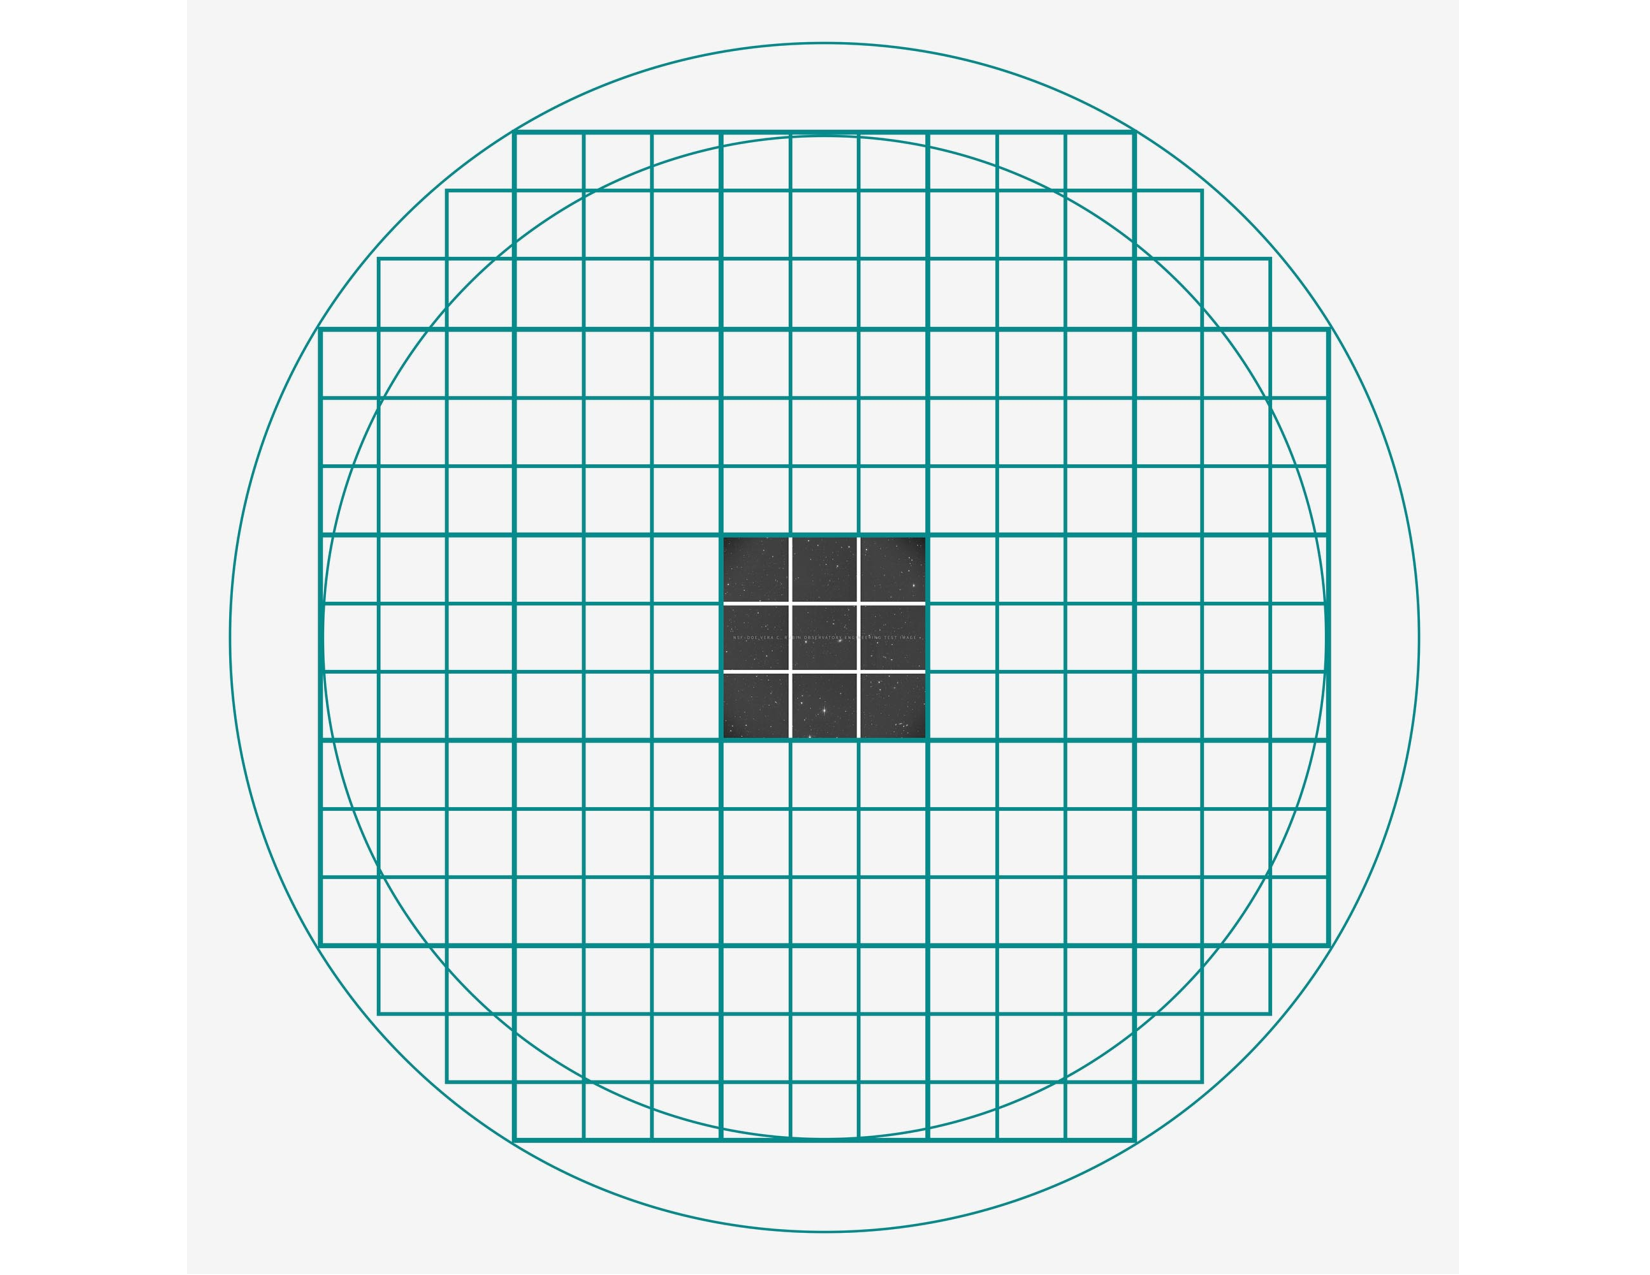
\includegraphics[width=0.98\linewidth]{commissioning/comcam_raft_in_lsstcam_focal_plane.pdf}
\caption{Schematic showing the single-raft \gls{LSSTComCam} positioned at the center of the full LSSTCam focal plane. The perspective is from above, looking down through the \gls{LSSTComCam} lenses onto the focal plane. Credit: RubinObs/NOIRLab/SLAC/NSF/DOE/AURA.}
\label{fig:comcam_raft_in_lsstcam_focal_plane}
\vspace{0.1cm}
\end{figure}

\figref{fig:comcam_focal_plane} shows the \gls{LSSTComCam} focal plane layout, illustrating the enumeration of sensors and amplifiers, along with their physical arrangement within the raft.
\begin{figure}[htb!]
\centering
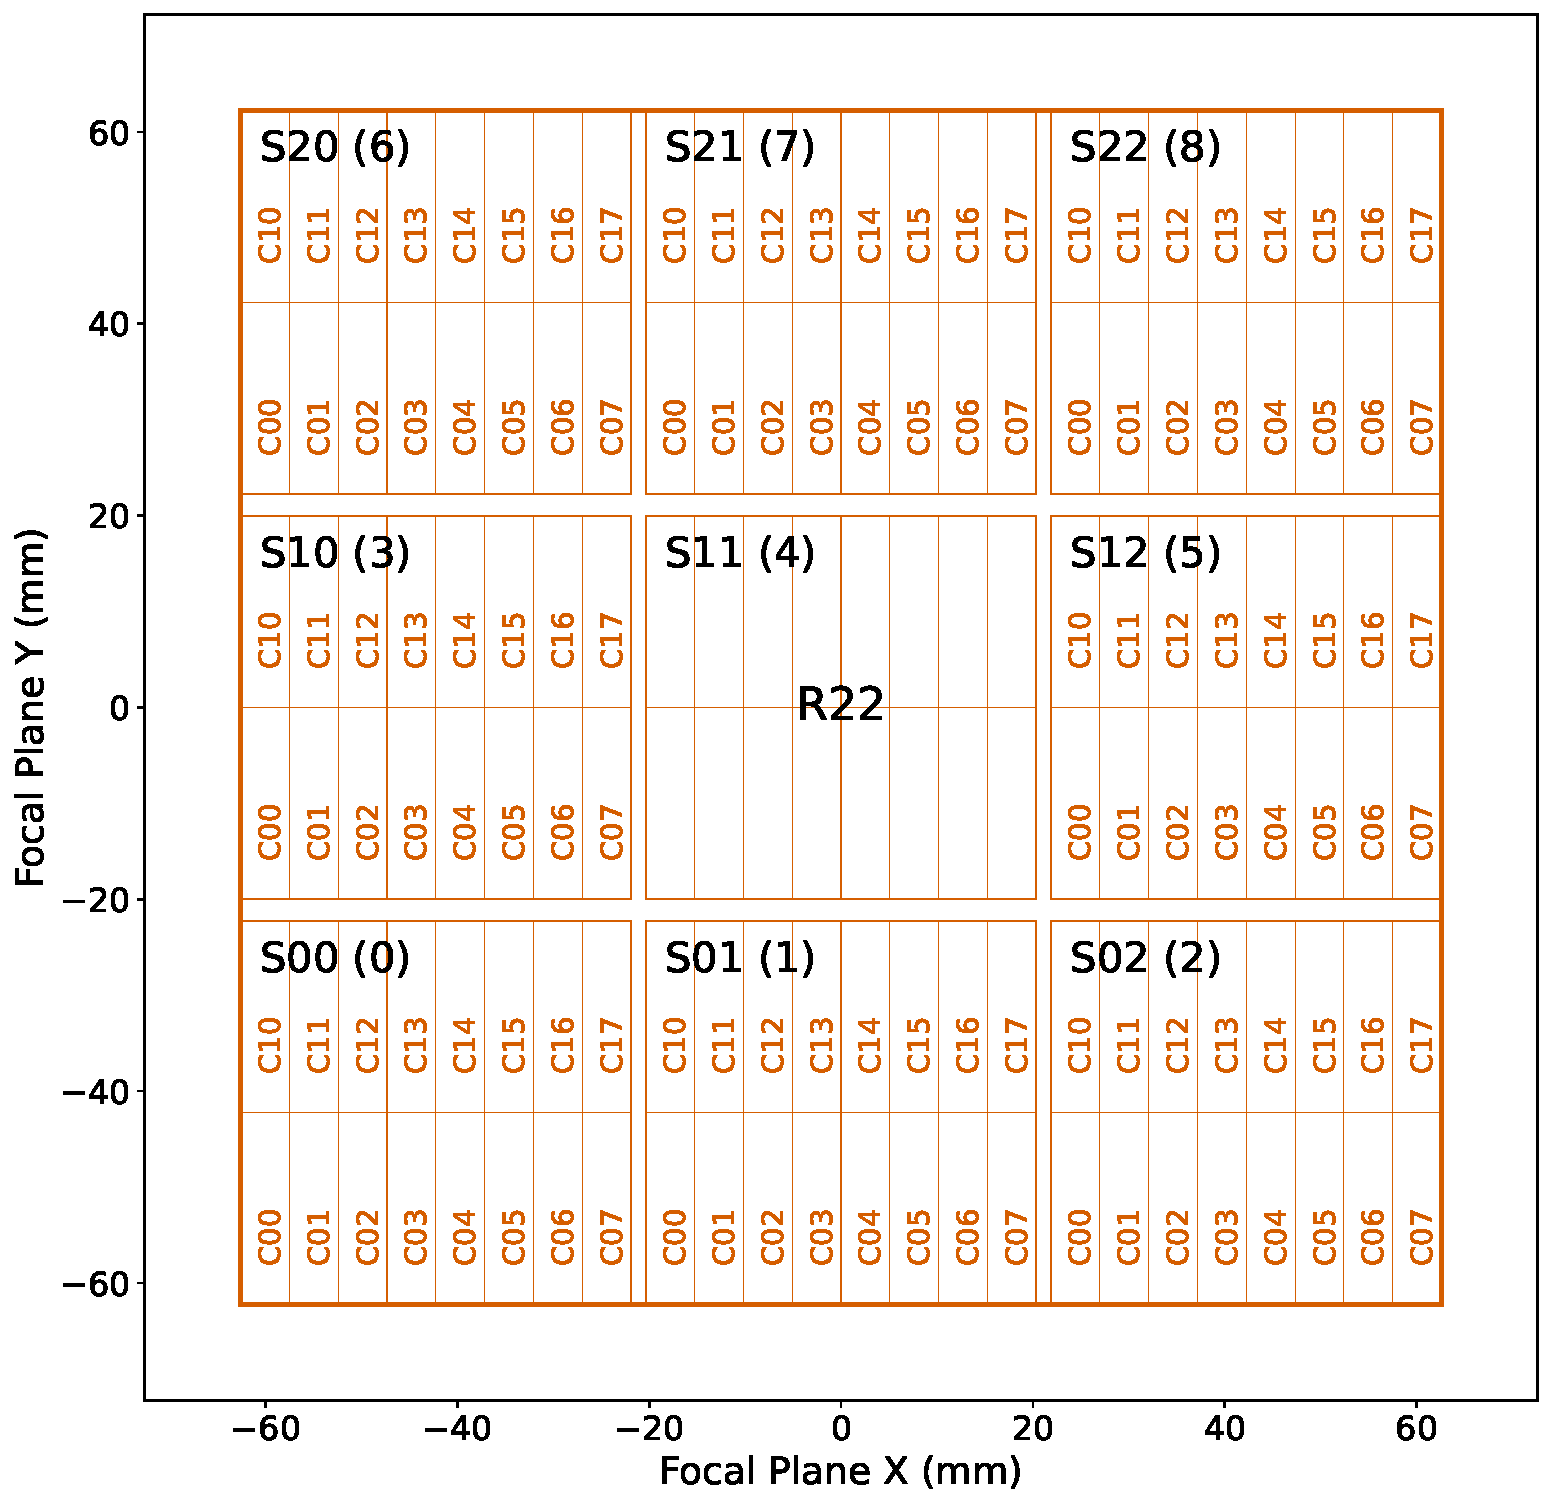
\includegraphics[width=\linewidth]{commissioning/comcam_focal_plane_schematic.pdf}
\caption{LSSTComCam focal plane layout illustrating the placement and numbering scheme of sensors (S) and amplifiers (C). The view is looking down from above the focal plane through the \gls{LSSTComCam} lenses. Each sensor contains 16 amplifiers, and a group of nine sensors comprises one raft. \gls{LSSTComCam} is Raft 22 (R22). The detector number for each sensor is shown in parentheses.}
\label{fig:comcam_focal_plane}
\vspace{0.1cm}
\end{figure}
The LSSTCam and \gls{LSSTComCam} focal planes are described in detail in \cite{ctn001}.

\gls{LSSTComCam} is housed in a support structure that precisely replicates the total mass, center of gravity, and physical dimensions of \gls{LSSTCam}, with all mechanical and utility interfaces to the telescope implemented identically.
This \gls{configuration} supports full end-to-end testing of the observatory systems, including readout electronics, image acquisition, and data pipelines.
The \gls{LSSTComCam} plate scale is \rawplatescale.

\subsubsection{Filter Complement}
\label{sssec:comcam_filters}
\gls{LSSTComCam} supports imaging with six broadband filters $ugrizy$ spanning 320–1050 nm, identical in design to \gls{LSSTCam}.
However, its filter exchanger can hold only three filters at a time, compared to five in \gls{LSSTCam}.
The full-system throughput of the six \gls{LSSTComCam} filters, which encompasses contributions from a standard atmosphere at airmass 1.2, telescope optics, camera surfaces, and the mean \gls{ITL} detector quantum efficiency is shown in \figref{fig:comcam_standard_bandpasses}.
\begin{figure}[htb!]
\centering
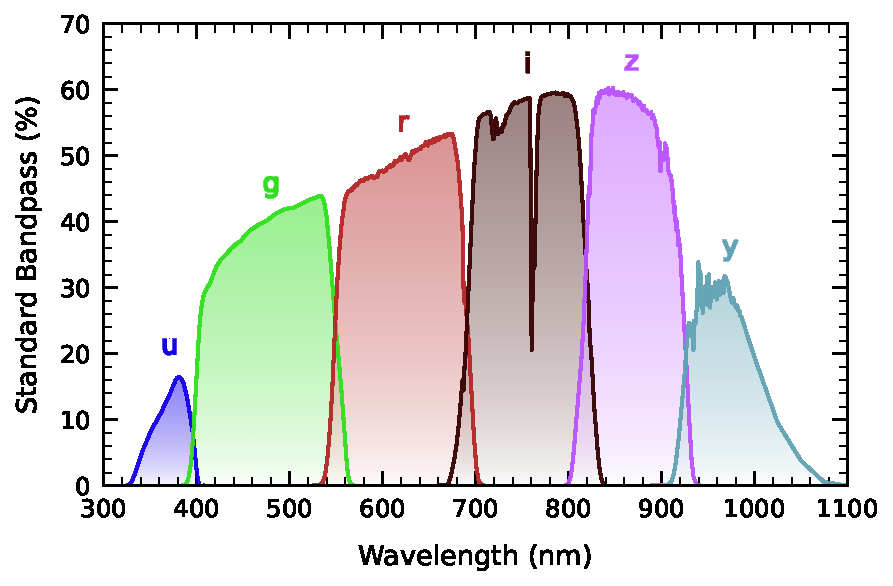
\includegraphics[width=0.98\linewidth]{commissioning/dp1_comcam_std_bandpasses.pdf}
\caption{LSSTComCam standard bandpasses, illustrating full system throughput. The bandpasses include a standard atmosphere at airmass 1.2, telescope optics, camera surfaces, and mean \gls{ITL} detector quantum efficiency.}
\label{fig:comcam_standard_bandpasses}
\vspace{0.1cm}
\end{figure}

% Reviewed by Eli
\subsection{Flat Field System
\label{ssec:flat_field_system}}
During the on-sky campaign, key components of the Rubin calibration system ~\citep{2022SPIE12182E..0RI}, including the flat field screen, \gls{CBP}, and the Ekspla tunable laser had not yet been installed.
As a result, flat fielding for \gls{DP1} relied entirely on twilight flats.
While twilight flats pose challenges such as non-uniform illumination and star print-through, they were the only available option during \gls{LSSTComCam} commissioning and for DP1 processing.
To mitigate these limitations, dithered, tracked exposures were taken over a broad range of azimuth and rotator angles to construct combined flat \gls{calibration} frames.
Exposure times were dynamically adjusted to reach target signal levels of between 10,000 and 20,000 electrons.
Future campaigns will benefit from more stable and uniform flat fielding using the Rubin flat field system, described in \citet{SITCOMTN-086}.

\subsection{LSST Science Pipelines Commissioning
\label{ssec:pipelines_commissioning}}
Commissioning of the \gls{LSST Science Pipelines} \citep{PSTN-019} began once the telescope was able to routinely deliver sub-arcsecond image quality.
The goals included testing the internal astrometric and photometric calibration across a range of observing conditions, validating the difference image analysis and Prompt Processing \citep{dmtn-219} framework, and accumulating over 200 visits per band to evaluate deep coadded images with integrated exposure times roughly equivalent to those of the planned LSST \gls{WFD} 10-year depth.
To support these goals, \nfields target fields were selected that span a range of stellar densities, overlap with external reference datasets, and collectively span the full breadth of the four primary \gls{LSST} science themes.
These \nfields fields form the basis of the \gls{DP1} dataset.
\figref{fig:dp1_fields_on_sky} shows the locations of these \nfields fields on the sky, overlaid on the LSST baseline survey footprint \citep{PSTN-051, PSTN-052, PSTN-053, PSTN-055, PSTN-056}, along with sky coverage of both the LSSTCam and \gls{LSSTComCam} focal planes.
\begin{figure*}[bt!]
\centering
\plotone{commissioning/dp1_fields_with_survey_fp}
\caption{Location of the seven DP1 fields overlaid on the \gls{LSST} baseline survey footprint. NES: North Ecliptic Spur, SCP: South Celestial Pole, Low-Dust WFD: regions away from the GP observed with a WFD cadence, GP/MC WFD: Galactic Plane and Magellanic Clouds regions observed with a WFD cadence. The \gls{FOV} covered by the \gls{LSSTCam} and \gls{LSSTComCam} focal planes is shown as concentric yellow circles about the pointing center of each field.}
\label{fig:dp1_fields_on_sky}
\end{figure*}
Each of the \nfields target fields was observed repeatedly in multiple bands over many nights.
A typical observing \gls{epoch} on a given target field consisted of 5-20 visits in each of the three loaded filters.
Only images taken as 1x30 second exposures have been included in \gls{DP1}.
All images were acquired using the Rubin \gls{FBS}, version 3.0 \citep{Naghib_2019, peter_yoachim_2024_13985198}.
\tabref{tab:dp1_fields} lists the \nfields \gls{DP1} fields and their pointing centers, and provides a summary of the band coverage in each.
\begin{deluxetable*}{llcccccccccr}
\tablecaption{DP1 fields and pointing centers with the number of exposures in each band per field. ICRS coordinates are in units of decimal degrees, and are specified as J2000.
\label{tab:dp1_fields}}
\tablehead{
  \colhead{\textbf{Field Code}} & 
  \colhead{\textbf{Field Name}} &
  \colhead{\textbf{RA}} & 
  \colhead{\textbf{DEC}} & 
  \colhead{} &  % spacer after DEC
  \multicolumn{6}{c}{\textbf{Band}} & 
  \colhead{\textbf{Total}} \\
  \cline{3-4} \cline{6-11}
  & & \colhead{deg} & \colhead{deg} & & 
  \colhead{$u$} & \colhead{$g$} & \colhead{$r$} & 
  \colhead{$i$} & \colhead{$z$} & \colhead{$y$} & \colhead{}
}
\startdata
47\_Tuc & \parbox[t]{6cm}{47 Tucanae Globular Cluster} & 6.128 & -72.090 & & 
\parbox{0.3cm}{6} & \parbox{0.3cm}{10} & \parbox{0.3cm}{32} & \parbox{0.3cm}{19} & \parbox{0.3cm}{0} & \parbox{0.3cm}{5} & 72 \\
ECDFS & \parbox[t]{6cm}{Extended Chandra Deep Field South} & 53.160 & -28.100 & & 
\parbox{0.3cm}{43} & \parbox{0.3cm}{230} & \parbox{0.3cm}{237} & \parbox{0.3cm}{162} & \parbox{0.3cm}{153} & \parbox{0.3cm}{30} & 855 \\
EDFS\_comcam & \parbox[t]{6cm}{Rubin SV Euclid Deep Field South} & 59.150 & -48.730 & & 
\parbox{0.3cm}{20} & \parbox{0.3cm}{61} & \parbox{0.3cm}{87} & \parbox{0.3cm}{42} & \parbox{0.3cm}{42} & \parbox{0.3cm}{20} & 272 \\
Fornax\_dSph & \parbox[t]{6cm}{Fornax Dwarf Spheroidal Galaxy} & 40.080 & -34.450 & & 
\parbox{0.3cm}{0} & \parbox{0.3cm}{5} & \parbox{0.3cm}{25} & \parbox{0.3cm}{12} & \parbox{0.3cm}{0} & \parbox{0.3cm}{0} & 42 \\
Rubin\_SV\_095\_-25 & \parbox[t]{6cm}{Rubin SV Low Galactic Latitude Field} & 95.040 & -25.000 & & 
\parbox{0.3cm}{33} & \parbox{0.3cm}{82} & \parbox{0.3cm}{84} & \parbox{0.3cm}{23} & \parbox{0.3cm}{60} & \parbox{0.3cm}{10} & 292 \\
Rubin\_SV\_38\_7 & \parbox[t]{6cm}{Rubin SV Low Ecliptic Latitude Field} & 37.980 & 7.015 & & 
\parbox{0.3cm}{0} & \parbox{0.3cm}{44} & \parbox{0.3cm}{40} & \parbox{0.3cm}{55} & \parbox{0.3cm}{20} & \parbox{0.3cm}{0} & 159 \\
Seagull & \parbox[t]{6cm}{Seagull Nebula} & 106.300 & -10.510 & & 
\parbox{0.3cm}{10} & \parbox{0.3cm}{37} & \parbox{0.3cm}{43} & \parbox{0.3cm}{0} & \parbox{0.3cm}{10} & \parbox{0.3cm}{0} & 100 \\
\hline
Total & & & & & 
\parbox{0.3cm}{112} & \parbox{0.3cm}{469} & \parbox{0.3cm}{548} & \parbox{0.3cm}{313} & \parbox{0.3cm}{285} & \parbox{0.3cm}{65} & 1792
\enddata
\end{deluxetable*}


The temporal sampling distribution of observations per band and per night is shown in \figref{fig:target_fields_temporal_sampling}.
Gaps in coverage across some bands arise from the fact that \gls{LSSTComCam} can only accommodate three filters at a time \secref{ssec:comcam}.
As the campaign progressed, the temporal sampling became denser across all fields, reflecting improved efficiency and increased time allocated for science observations.
The \gls{ECDFS} field received the most consistent and densest temporal sampling.
It is important to note that the time sampling in the \gls{DP1} dataset differs significantly from what will be seen in the final \gls{LSST} data.
\begin{figure*}[htb!]
\centering
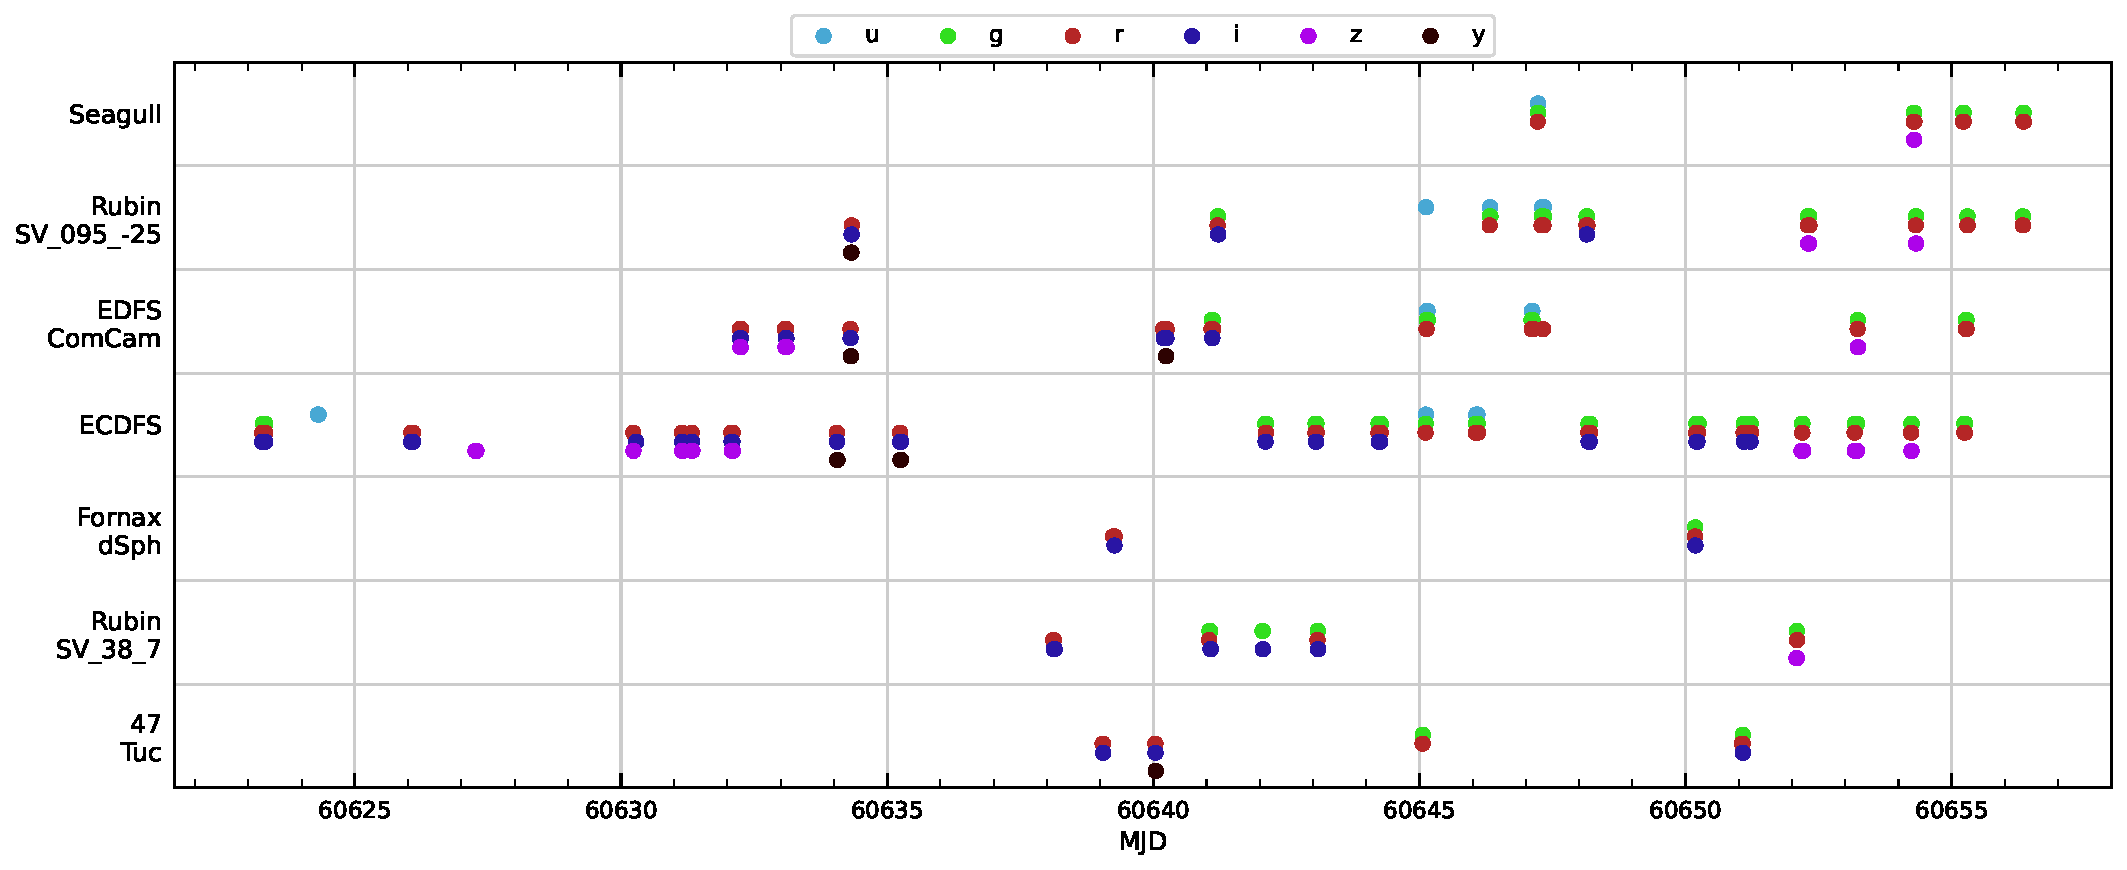
\includegraphics[width=1.0\linewidth]{commissioning/temporal_sampling_per_field.pdf}
\caption{Distribution of \gls{DP1} observations by date grouped by field and color coded by band.}
\label{fig:target_fields_temporal_sampling}
\vspace{0.1cm}
\end{figure*}

% Spatial coverage  -- are these needed given figure 1?
% \figref{fig:dp1_fields_coverage} shows the sky coverage for each of the \nfields DP1 fields.
All fields except for the low ecliptic latitude field, Rubin\_SV\_38\_7, used random translational and rotational dithers within a 0.2 degree radius around the pointing center (\tabref{tab:dp1_fields}).
The rotational dithers were typically applied at the time of filter changes for operational efficiency, with translational dithers of approximately 1 degree applied between individual visits.
\begin{figure*}[ht]
    \centering
    \begin{subfigure}[t]{0.3\textwidth}
        \centering
        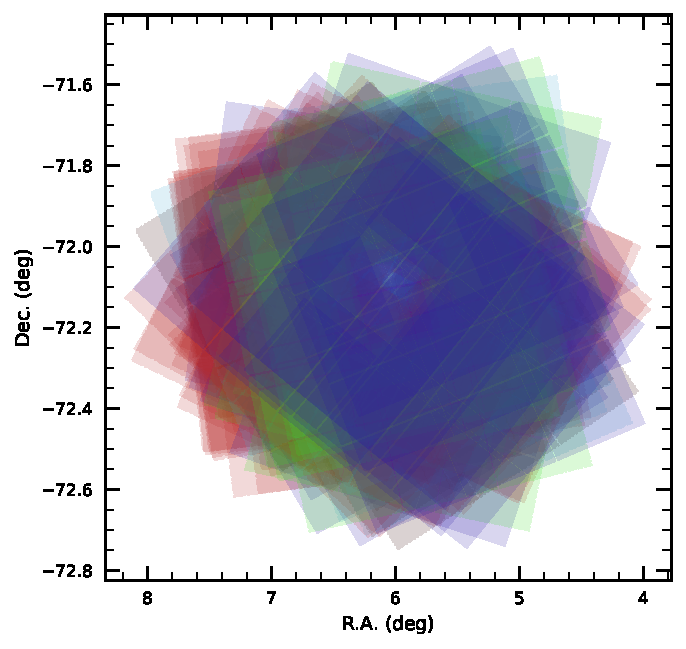
\includegraphics[width=\linewidth]{visitskymaps/showVisit_DP1_47Tuc}
        \caption{47 Tucanae}
    \end{subfigure}\hfill
    \begin{subfigure}[t]{0.3\textwidth}
        \centering
        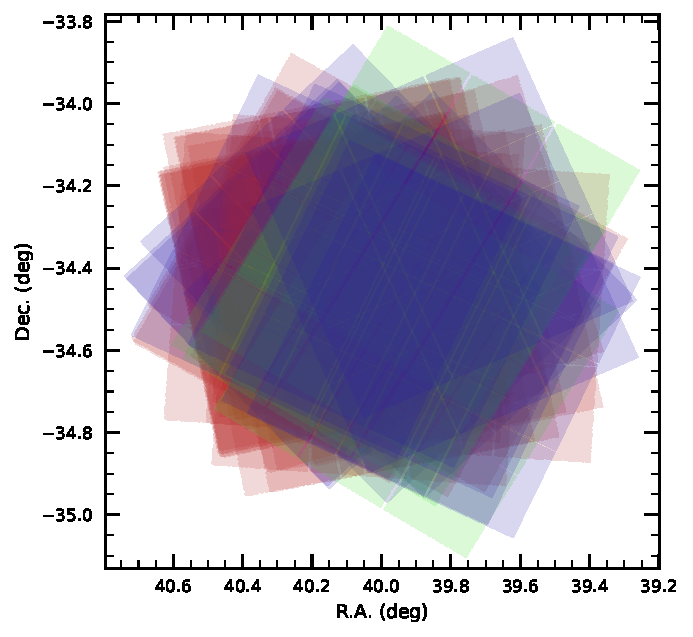
\includegraphics[width=\linewidth]{visitskymaps/showVisit_DP1_Fornax_dSph}
        \caption{Fornax dwarf Spheroidal}
    \end{subfigure}\hfill
    \begin{subfigure}[t]{0.3\textwidth}
        \centering
        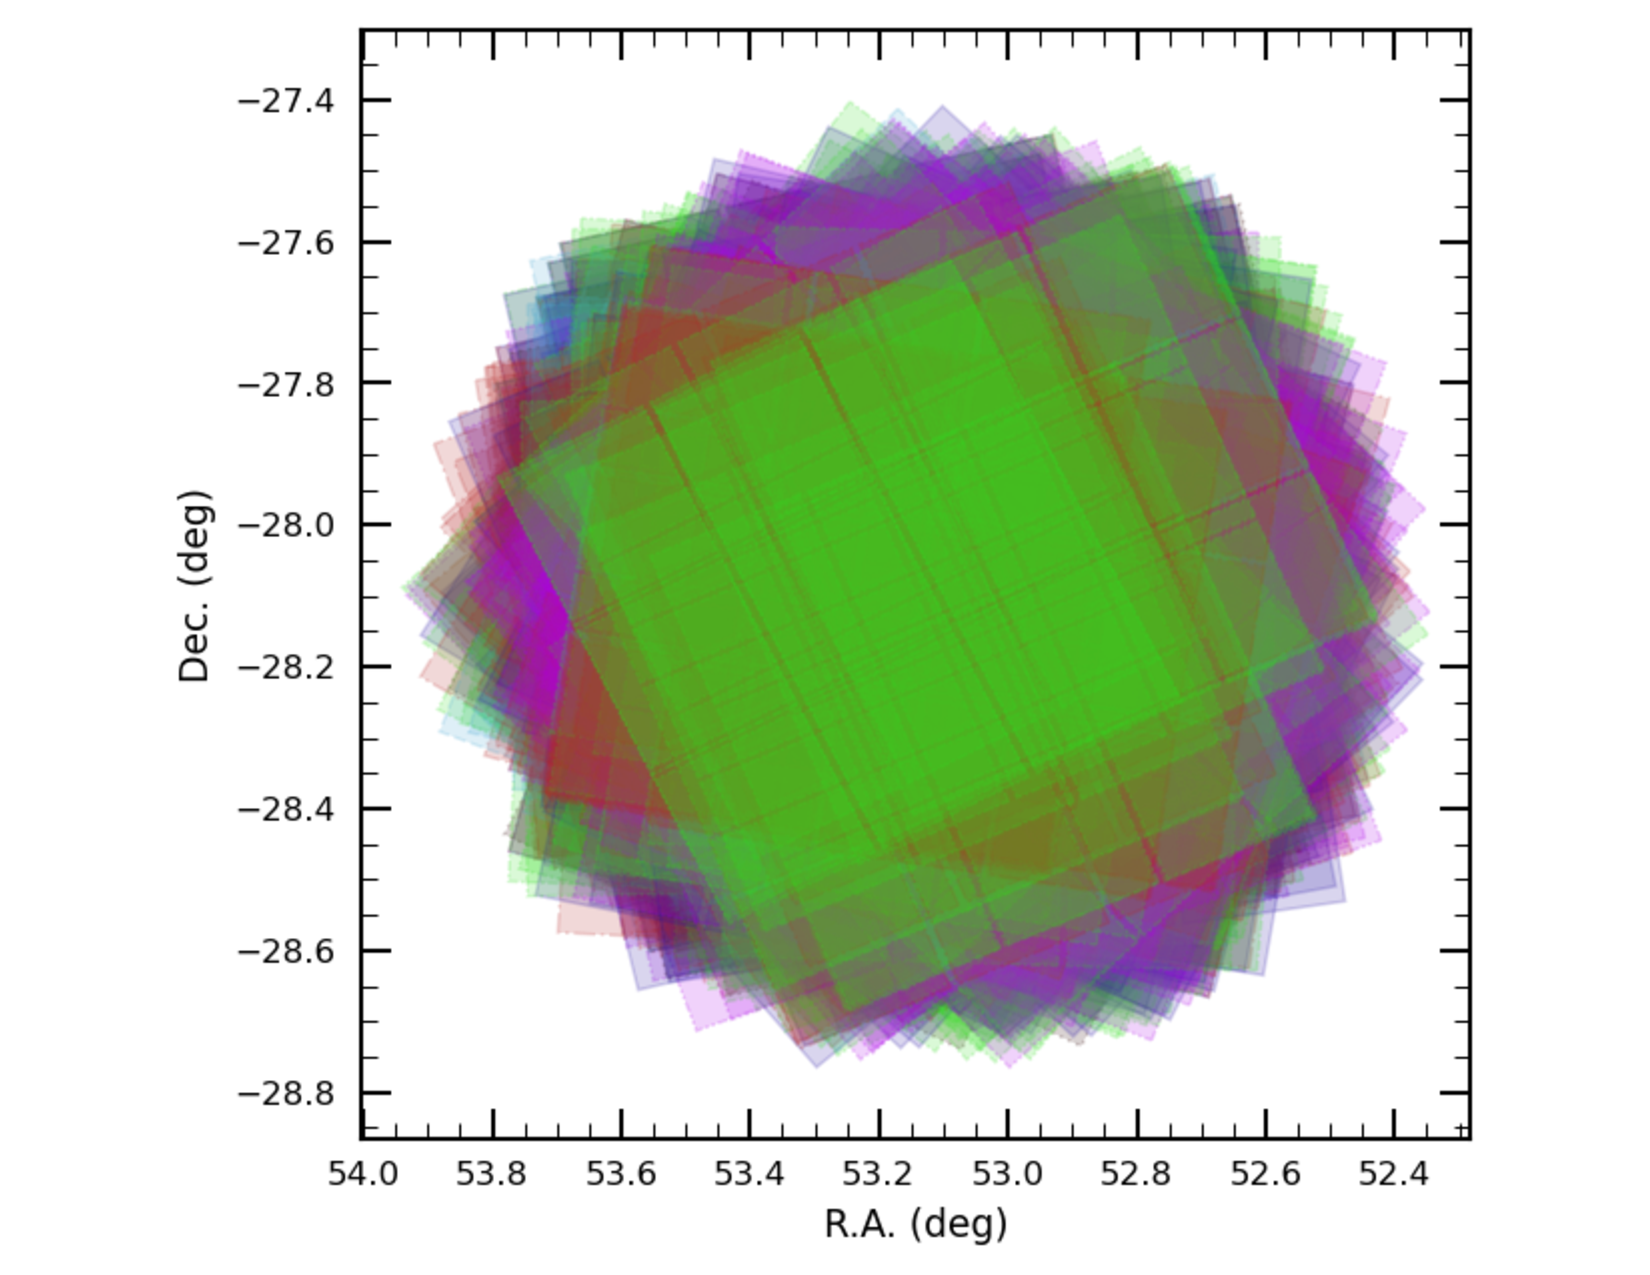
\includegraphics[width= \linewidth]{visitskymaps/showVisit_DP1_ECDFS}
        \caption{ECDFS}
    \end{subfigure}
    \vspace{1em}

    % Row 2
    \begin{subfigure}[t]{0.3\textwidth}
        \centering
        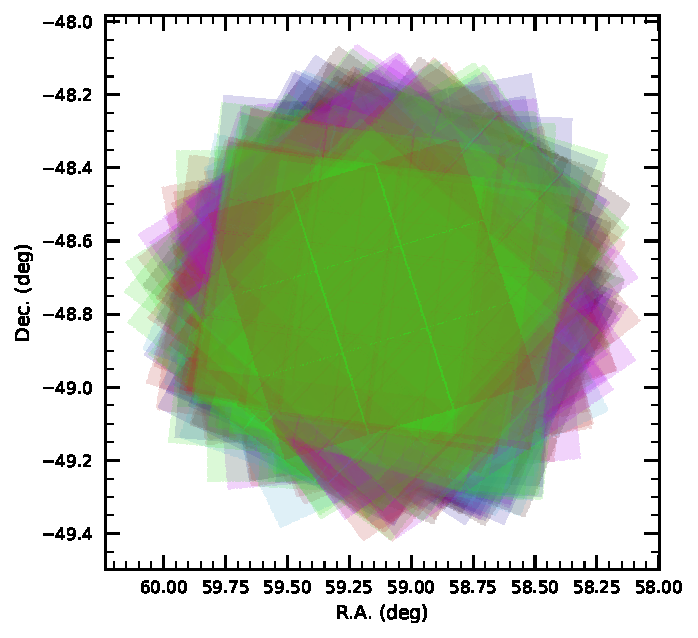
\includegraphics[width=\linewidth]{visitskymaps/showVisit_DP1_EDFS}
        \caption{EDFS}
    \end{subfigure}\hfill
    \begin{subfigure}[t]{0.3\textwidth}
        \centering
        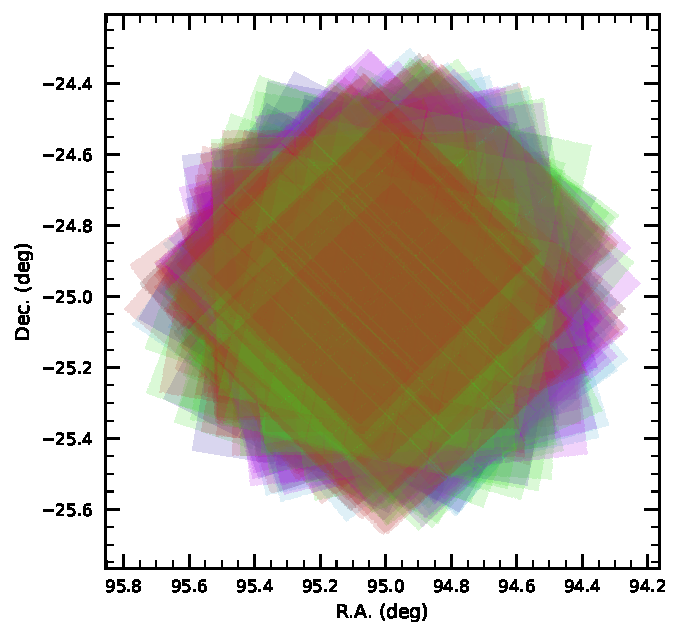
\includegraphics[width=\linewidth]{visitskymaps/showVisit_DP1_RubinSV_95_-25}
        \caption{RubinSV\_95\_-25}
    \end{subfigure}\hfill
    \begin{subfigure}[t]{0.3\textwidth}
        \centering
        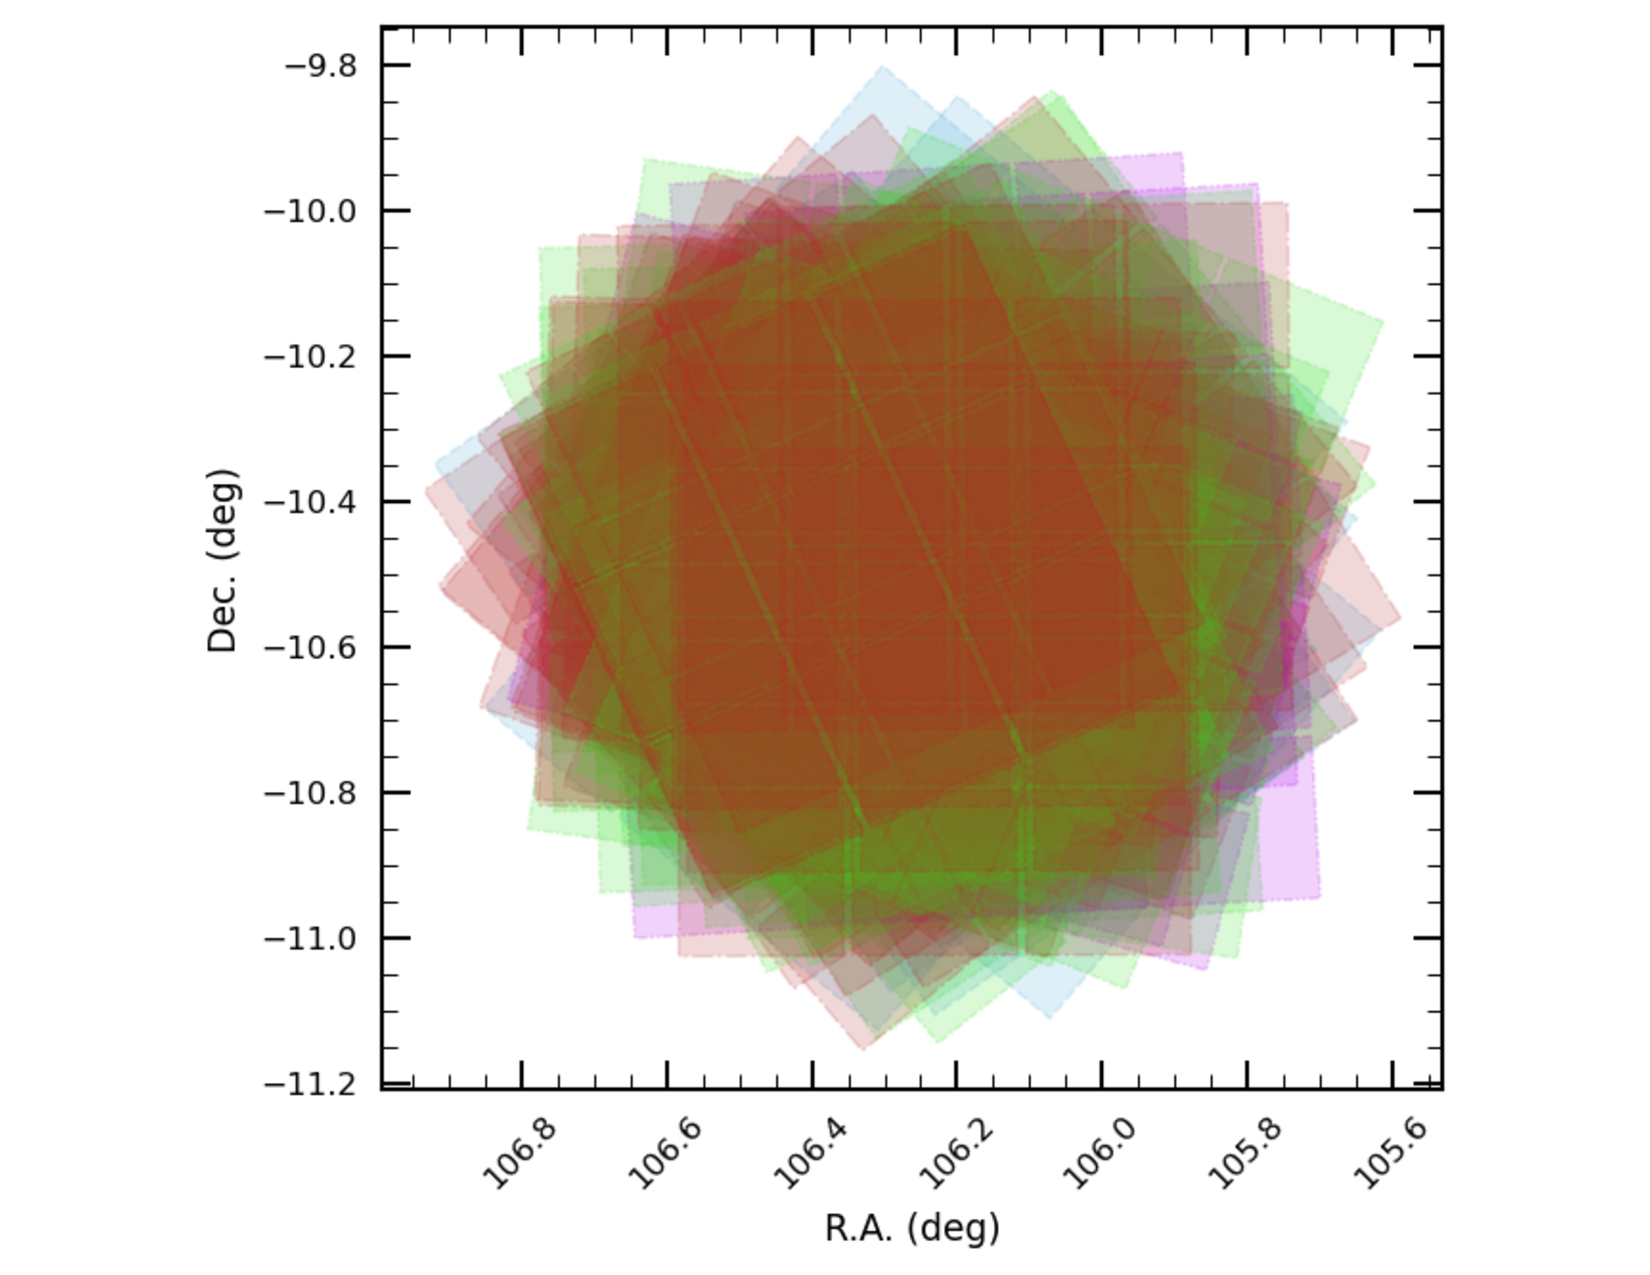
\includegraphics[width= \linewidth]{visitskymaps/showVisit_DP1_Seagull}
        \caption{Seagull}
    \end{subfigure}
    \vspace{1em}

    % Row 3
    \hspace*{0.3\textwidth} % Empty left slot
    \begin{subfigure}[t]{0.29\textwidth}
        \centering
        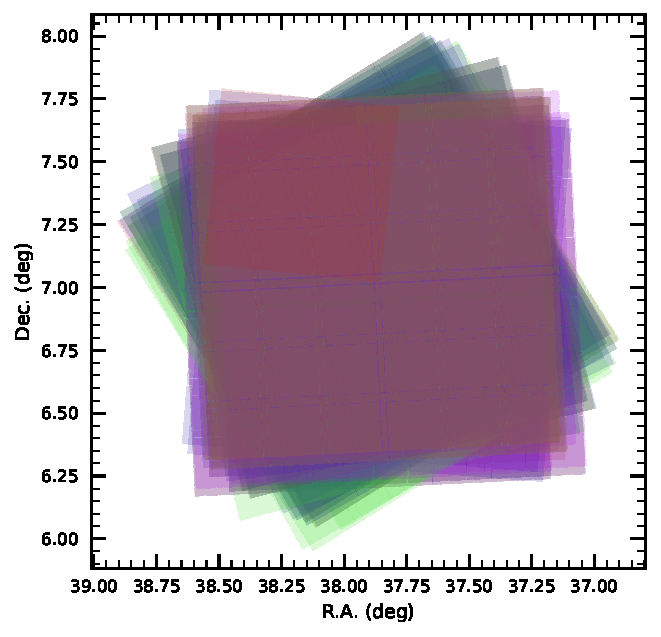
\includegraphics[width=\linewidth]{visitskymaps/showVisit_DP1_RubinSV_38_7}
        \caption{Rubin\_SV\_38\_7}
    \end{subfigure}
    \hspace{0.3\textwidth} % Empty left slot
    \vspace{1em}

    \caption{Sky coverage for seven \gls{DP1} fields.}
    \label{fig:dp1_fields_coverage}
\end{figure*}
The Rubin\_SV\_38\_7 field used a different dither pattern to optimize coverage of Solar System Objects and test Solar System \gls{Object} linking across multiple nights.
These observations used a 2 x 2 grid of \gls{LSSTComCam} pointings to cover an area of about 1.3 degree x 1.3 degrees.
The visits cycled between the grid’s four pointing centers, using small random dithers to fill chip gaps with the goal of acquiring 3-4 visits per pointing center per band in each observing \gls{epoch}.

% PSF limiting magnitude
% \figref{fig:dp1_fields_depth} shows the
% resulting integrated depth, expressed in terms of the flux of an unresolved source that would
% be measured with signal-to-noise ratio S/N = 5 in the r-band.
% \begin{figure*}[ht]
%     \centering
%     \begin{subfigure}[t]{0.3\textwidth}
%         \centering
%         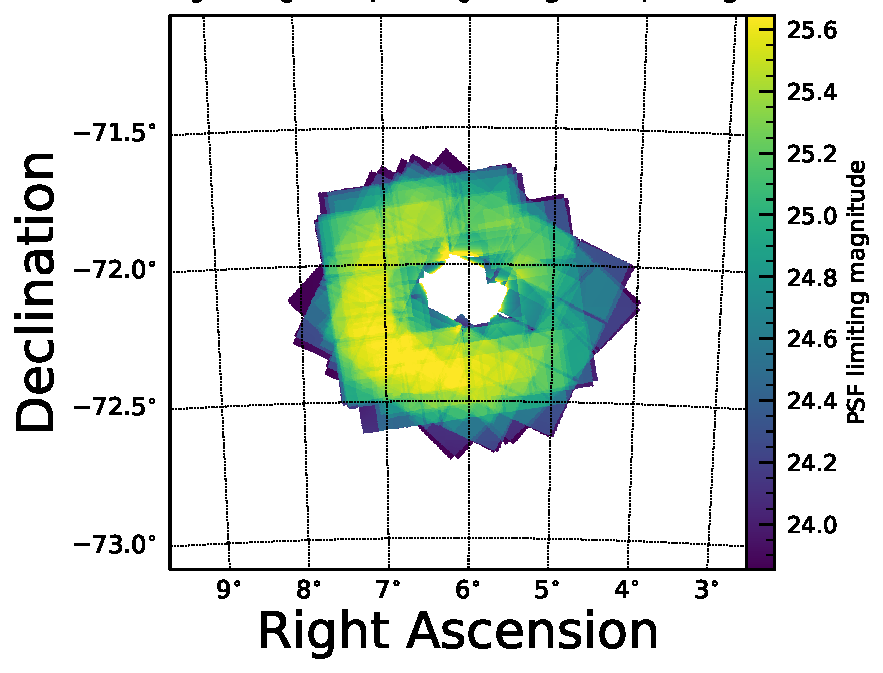
\includegraphics[width=\linewidth]{figures/maglim/DP1_47_Tuc_psf_maglim_r.pdf}
%         \caption{47 Tucanae}
%     \end{subfigure}\hfill
%     \begin{subfigure}[t]{0.3\textwidth}
%         \centering
%         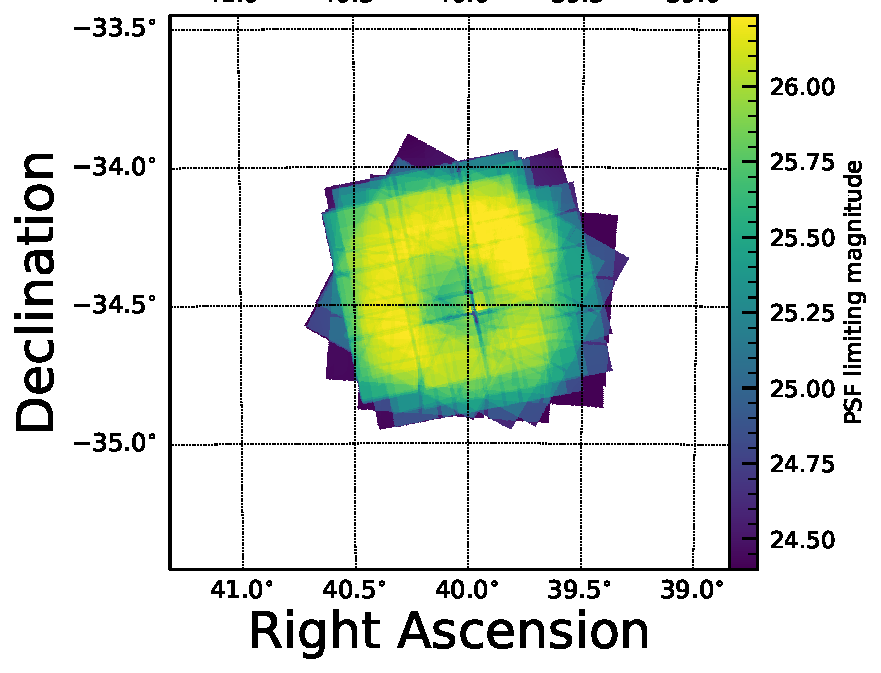
\includegraphics[width=\linewidth]{figures/maglim/DP1_Fornax_dSph_psf_maglim_r.pdf}
%         \caption{Fornax dwarf Spheroidal}
%     \end{subfigure}\hfill
%     \begin{subfigure}[t]{0.3\textwidth}
%         \centering
%         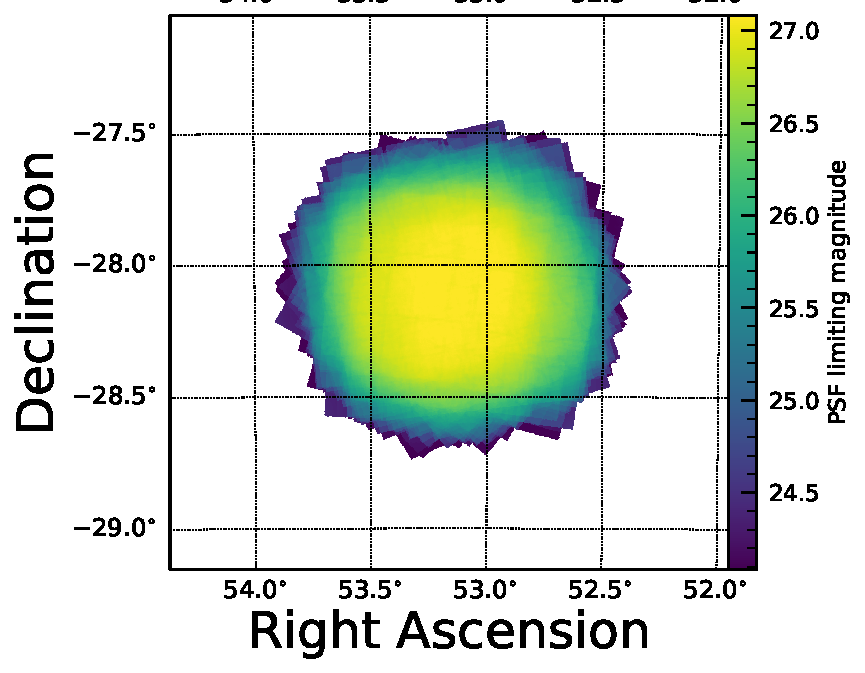
\includegraphics[width= \linewidth]{figures/maglim/DP1_ECDFS_psf_maglim_r.pdf}
%         \caption{ECDFS}
%     \end{subfigure}
%     \vspace{1em}

%     % Row 2
%     \begin{subfigure}[t]{0.3\textwidth}
%         \centering
%         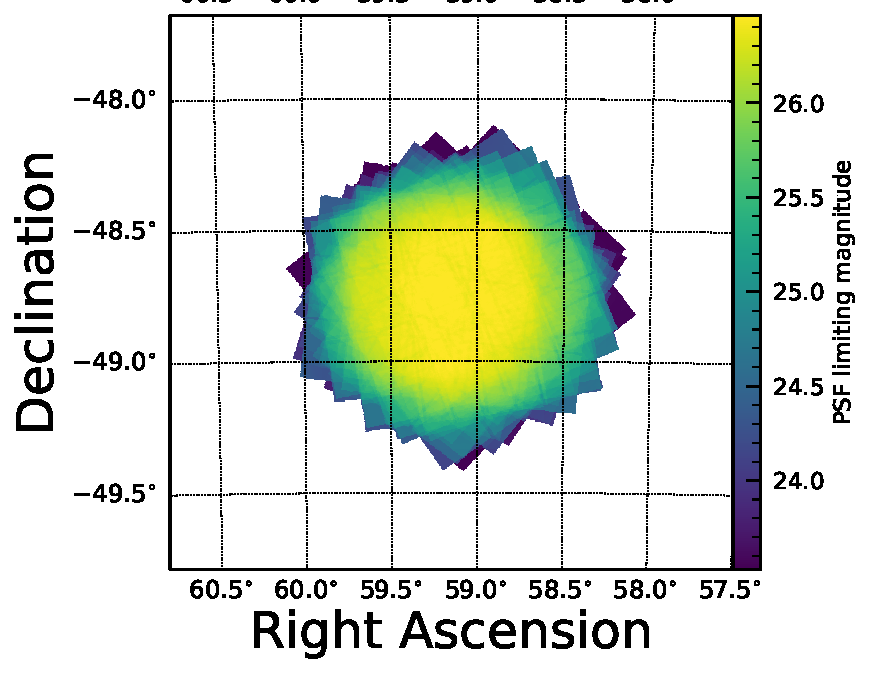
\includegraphics[width=\linewidth]{figures/maglim/DP1_EDFS_comcam_psf_maglim_r.pdf}
%         \caption{EDFS}
%     \end{subfigure}\hfill
%     \begin{subfigure}[t]{0.3\textwidth}
%         \centering
%         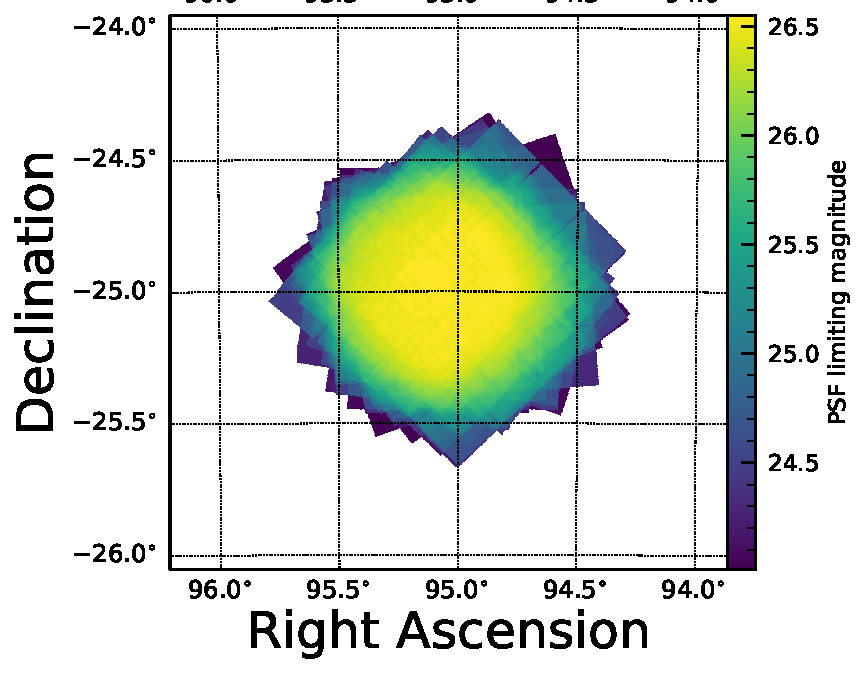
\includegraphics[width=\linewidth]{figures/maglim/DP1_Rubin_SV_095_-25_psf_maglim_r.pdf}
%         \caption{RubinSV\_95\_-25}
%     \end{subfigure}\hfill
%     \begin{subfigure}[t]{0.3\textwidth}
%         \centering
%         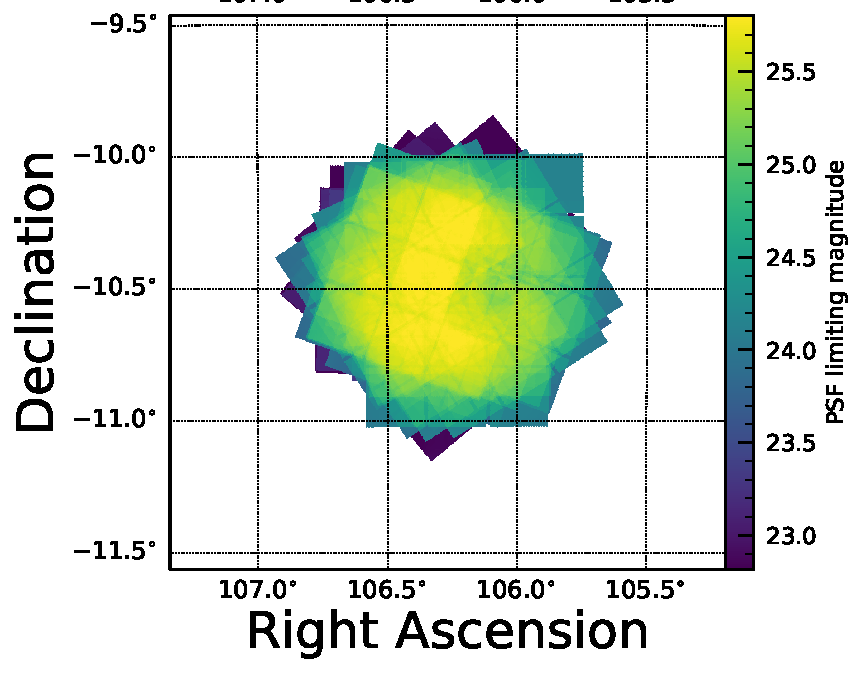
\includegraphics[width=\linewidth]{figures/maglim/DP1_Seagull_psf_maglim_r.pdf}
%         \caption{Seagull}
%     \end{subfigure}
%     \vspace{1em}

%     % Row 3
%     \hspace{0.3\textwidth}
%     \begin{subfigure}[t]{0.29\textwidth}
%         \centering
%         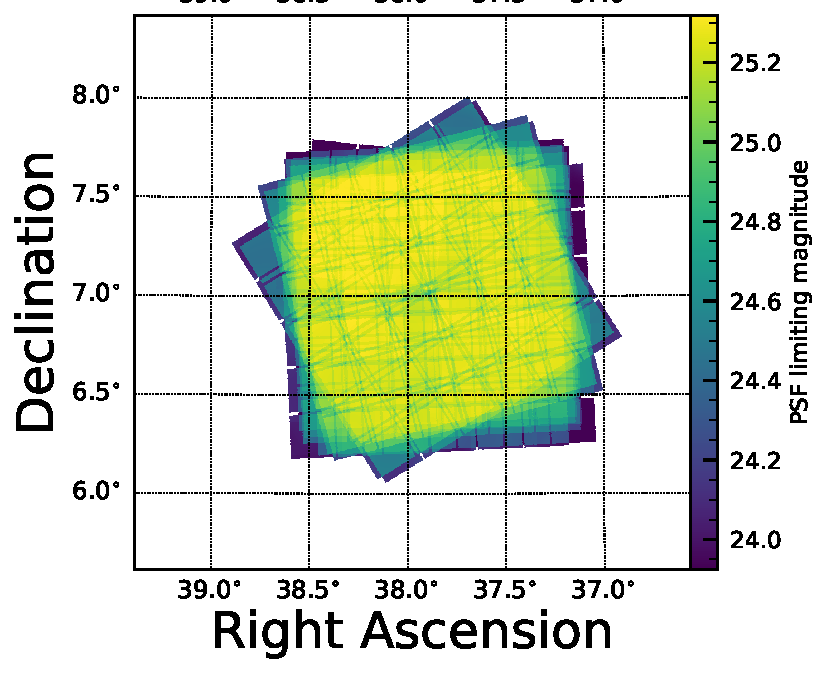
\includegraphics[width=\linewidth]{figures/maglim/DP1_Rubin_SV_38_7_psf_maglim_r.pdf}
%         \caption{Rubin\_SV\_38\_7}
%     \end{subfigure}
%     \hspace*{0.3\textwidth}
%     \caption{Cumulative imaging depth expressed in terms of the S/N = 5 limiting r-band magnitude for unresolved sources in the seven DP1 fields.}
%     \label{fig:dp1_fields_depth}
% \end{figure*}

% Reviewed by Elana
\subsection{Delivered Image Quality
\label{ssec:image_quality}}
The delivered image quality is influenced by contributions from both the observing system (i.e., dome, telescope and \gls{camera}) and the atmosphere.
During the campaign, the Rubin \gls{DIMM} was not operational, so atmospheric seeing was estimated using live data from the \gls{SOAR} \gls{RINGSS} seeing monitor.
Although accelerometers mounted on the mirror cell and top-end assembly were available to track dynamic optics effects, such as mirror oscillations that can degrade optical alignment, this data was not used during the campaign.
Mount encoder data was used to measure the mount jitter in every image, with a median contribution of 0.004 arcseconds to image degradation measured.
As the pointing model was not fine tuned, tracking errors could range from 0.2 to 0.4 arcseconds per image, depending on RA and Dec.
%RA resolves to Rapid Analysis
Dome and mirror-induced \gls{seeing} were not measured during the campaign.
% Not sure this is needed
% %%%%% This table is auto generated from data, DO NOT EDIT
\setlength{\tabcolsep}{14pt} 
\begin{deluxetable*}{ccccc}
\tablecaption{Image quality expressed in terms of PSF FWHM in arcseconds per band and for all bands.
\label{tab:image_quality} }
\tablehead{
  \colhead{\textbf{Band}} && \multicolumn{3}{c}{\textbf{Quantile (\%)}} \\
  \cline{3-5}
   & & 25& 50& 75 
}
\startdata
u &   & 1.34 & 1.48 & 1.67 \\
g &   & 1.07 & 1.17 & 1.29 \\
r &   & 0.99 & 1.12 & 1.22 \\
i &   & 0.92 & 1.03 & 1.13 \\
z &   & 0.98 & 1.11 & 1.21 \\
y &   & 0.94 & 1.01 & 1.10 \\
all &   & 1.00 & 1.13 & 1.25 \\
\enddata
\end{deluxetable*}
% \tabref{tab:image_quality} summarizes the delivered image quality expressed in terms of the PSF FWHM in arcseconds per band for the \nexposures in DP1.
The median delivered image quality for commanded in-focus images (all bands) was \medianimagequalityallbands, as measured by the \gls{PSF} \gls{FWHM}.
The best images achieved a \gls{PSF} \gls{FWHM} of approximately \bestimagequality.
\begin{figure}[htb!]
\centering
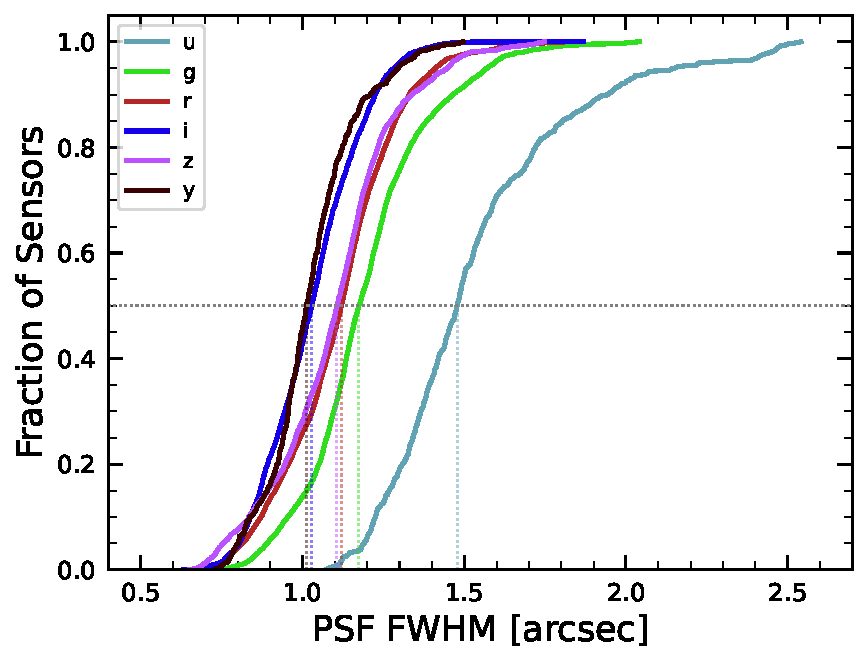
\includegraphics[width=0.98\linewidth]{commissioning/image_quality_ecdf.pdf}
\caption{Cumulative distribution of \gls{PSF} \gls{FWHM} of the \gls{DP1} dataset.}
\label{fig:delivered_image_quality_ecdf}
\end{figure}
Ongoing efforts aim to quantify all sources of image degradation,  including contributions from the \gls{camera} system, static and dynamic optical components, telescope mount motion,  observatory-induced seeing from the dome and mirror, and atmospheric conditions.

